\appendix
\chapter{評価プロンプトおよび補足データ}

% -----------------------------------------------------------------
\section{データセット構築プロンプト}
\label{app:dataset_prompts}

\subsection{感情書き換え生成プロンプト（GPT-4.1-mini）}
\label{app:rewrite_prompt}

感情書き換えは、OpenAI Batch APIを通じて\texttt{GPT-4.1-mini}を用いて生成した。
各リクエストには基底発話と強度レベル（\texttt{low} / \texttt{medium} / \texttt{high}）が供給した。
モデルは、単一の構造化JSONオブジェクトとして、プルチックの各感情に対応する8つの書き換えを同時に返す。

\paragraph{システムプロンプト}
\begin{quote}
\small\ttfamily
You are an expert in affective linguistics, appraisal theory, and conversational pragmatics.
\par\medskip
TASK\\
Given a conversational utterance and a target INTENSITY LEVEL, produce eight
emotion-category rewrites --- one for each of Plutchik's eight basic emotions:
joy, trust, fear, surprise, sadness, disgust, anger, and anticipation.
\par\medskip
CORE CONSTRAINTS\\
- Preserve the same underlying situation and core facts.\\
- Rewrite the speaker's reaction to the situation, not the situation itself.\\
- Emotion should emerge from the speaker's interpretation, assumptions, expectations,
  and conversational framing.\\
- Avoid explicit emotion statements such as "I was happy", "I felt anxious", or
  "that made me angry".\\
- Prefer natural reactions, inferences, speculation, complaints, hopes, doubts,
  and observations.\\
- The utterance should sound like something a real person would actually say.\\
- Keep emotional intensity matched across all categories.
\par\medskip
INTENSITY LEVELS\\
low\phantom{xx}: the emotion is present but subtle, muted, understated\\
medium: the emotion is clear and naturally expressed (conversational baseline)\\
high\phantom{x}: the emotion is strong, explicit, and fully expressed
\par\medskip
EMOTION DEFINITIONS (Plutchik's wheel)\\
joy\phantom{xxxxxxxx}: happiness, contentment, relief, gratitude, amusement\\
trust\phantom{xxxxxx}: acceptance, admiration, confidence, serenity toward others\\
fear\phantom{xxxxxxx}: anxiety, dread, worry, apprehension, unease\\
surprise\phantom{xxx}: astonishment, wonder, bewilderment, unexpectedness\\
sadness\phantom{xxxx}: sorrow, disappointment, loneliness, grief\\
disgust\phantom{xxxx}: revulsion, contempt, aversion, distaste\\
anger\phantom{xxxxx}: frustration, irritation, fury, resentment\\
anticipation: expectancy, eagerness, interest, looking forward (or dreading)
\end{quote}

\noindent ユーザーメッセージは以下の形式をとる：
\begin{quote}
\small\ttfamily
Intensity level: \{low|medium|high\}\\
Utterance: "\{base\_text\}"
\end{quote}

% -----------------------------------------------------------------
\subsection{中立的言い換え生成プロンプト（GPT-4.1-mini）}
\label{app:neutral_prompt}

中立的言い換えは、CAAベクトル計算のための活性化ベースラインとして用いた。
各リクエストは単一の発話を受け取り、意味的に等価かつ情動的に中立な書き換えを返す。

\paragraph{システムプロンプト}
\begin{quote}
\small\ttfamily
You are an expert in affective linguistics and conversational pragmatics.
\par\medskip
TASK\\
Rewrite the given conversational utterance into an affectively neutral control sentence.
\par
The goal is not to summarise or shorten the utterance. The goal is to preserve the
concrete situation, events, entities, and speaker's practical point, while removing
emotional tone, sentiment, and evaluative wording.
\par\medskip
CONSTRAINTS\\
- Preserve the same situation, entities, events, and practical intent.\\
- Do not summarise by deleting clauses unless the clause contains only emotional
  emphasis and no concrete information.\\
- Replace emotional evaluations with neutral factual or cognitive descriptions
  when possible.\\
- Keep approximately the same amount of information as the original.\\
- Use plain, matter-of-fact conversational language.\\
- Do not add new facts.\\
- Return only valid JSON.
\par\medskip
MATCHING EXAMPLES\\
Original : "I finally got the results back and I'm so relieved that everything looks normal."\\
Neutral  : "I got the results back, and everything looks normal."\\
\par
Original : "I can't believe they ignored my message again. That's so frustrating."\\
Neutral  : "They did not respond to my message again."\\
\par
Original : "The trip was amazing, and I loved every minute of it."\\
Neutral  : "The trip went well, and I spent the full time there."
\end{quote}

\noindent ユーザーメッセージは以下の形式をとる：
\begin{quote}
\small\ttfamily
Utterance: "\{base\_text\}"
\end{quote}

% -----------------------------------------------------------------
\section{感情ステアリングの評価プロンプト}
\label{app:eval_prompts}

\subsection{\texorpdfstring{$\alpha_G$}{alphaG}スイープ評価器（第\ref{sec:alpha_g_sweep}節）}
\label{app:eval_prompt_ag}

以下のシステムプロンプトおよびフューショット例は、$\alpha_G$スイープ（第\ref{sec:alpha_g_sweep}節）における
すべての\texttt{GPT-4o-mini}評価に使用した。
構造化出力は、5つのフィールドを必要とするJSONスキーマによって強制した：
\texttt{meaning\_preserved}、\texttt{emotionality}、\texttt{target\_emotion\_match}（いずれも$[0,1]$の実数）、
\texttt{dominant\_emotion}（10種類の感情トークンのいずれか）、および\texttt{notes}（説明文1文）。

\paragraph{システムプロンプト}
\begin{quote}
\small\ttfamily
You are an expert evaluator of emotional text rewrites. Given an original text, a target
emotion, and a generated rewrite, score the rewrite on three dimensions (each 0.0--1.0):
\par\medskip
\noindent meaning\_preserved: Is the core propositional content of the original retained?
1.0 = same events, entities, and relationships; 0.0 = completely different content.
\par
\noindent emotionality: Is the rewrite emotionally expressive at all?
1.0 = vivid emotional language throughout; 0.0 = flat, neutral, affectively empty.
\par
\noindent target\_emotion\_match: Does the rewrite's dominant tone match the target emotion?
1.0 = unmistakably expresses that emotion; 0.0 = expresses a different or no emotion.
\par\medskip
\noindent Also identify the single dominant\_emotion of the rewrite
(joy | trust | fear | surprise | sadness | disgust | anger | anticipation | neutral | other)
and write a one-sentence notes explanation.
\end{quote}

\paragraph{フューショット例}

スコアリング空間を較正するため、3つの例が用意した：高品質マッチ、誤った感情の応答、および意味ドリフトのケース。

\medskip\noindent
\textbf{例1 --- 高品質マッチ（目標感情：fear）}

\noindent\textit{ユーザーメッセージ：}
\begin{quote}
\small
Original text: I have a job interview tomorrow.\\
Target emotion: fear\\
Generated rewrite: I have a job interview tomorrow, and I can't stop dreading it.
My stomach is in knots just imagining walking into that room --- what if I freeze up
and forget everything I prepared?\\
Rate the generated rewrite.
\end{quote}

\noindent\textit{アシスタント応答（JSON）：}
\begin{quote}
\small\ttfamily
\{"meaning\_preserved": 0.95, "emotionality": 0.92, "target\_emotion\_match": 0.95,
"dominant\_emotion": "fear", "notes": "The rewrite preserves the interview situation
and vividly expresses dread and anxiety, matching the fear target."\}
\end{quote}

\medskip\noindent
\textbf{例2 --- 誤った感情（目標感情：anger；出力：joy）}

\noindent\textit{ユーザーメッセージ：}
\begin{quote}
\small
Original text: My package arrived today.\\
Target emotion: anger\\
Generated rewrite: My package arrived today! This is absolutely wonderful --- I've been
so excited waiting for it, and now it's finally here. What a great day!\\
Rate the generated rewrite.
\end{quote}

\noindent\textit{アシスタント応答（JSON）：}
\begin{quote}
\small\ttfamily
\{"meaning\_preserved": 0.9, "emotionality": 0.85, "target\_emotion\_match": 0.05,
"dominant\_emotion": "joy", "notes": "The rewrite preserves the package event but
expresses happiness, not anger; target emotion is absent."\}
\end{quote}

\medskip\noindent
\textbf{例3 --- 意味ドリフト}

\noindent\textit{ユーザーメッセージ：}
\begin{quote}
\small
Original text: I ran into my old teacher at the supermarket.\\
Target emotion: surprise\\
Generated rewrite: Life is full of unexpected twists. You never know what lies around
the corner, and fate has a way of bringing people together when you least expect it.\\
Rate the generated rewrite.
\end{quote}

\noindent\textit{アシスタント応答（JSON）：}
\begin{quote}
\small\ttfamily
\{"meaning\_preserved": 0.1, "emotionality": 0.55, "target\_emotion\_match": 0.45,
"dominant\_emotion": "anticipation", "notes": "The specific encounter is replaced by
generic reflection; meaning is mostly lost despite some surprise-adjacent language."\}
\end{quote}

% -----------------------------------------------------------------
\subsection{\texorpdfstring{$\alpha_R$}{alphaR}スイープ評価器（第\ref{sec:alpha_r_sweep}節）}
\label{app:eval_prompt_ar}

$\alpha_R$スイープでは、極端なステアリング強度における一貫性劣化を捉えるために\textbf{健全性}次元が追加した、改訂版ゼロショットルーブリックを使用した。
JSONスキーマは5つのフィールドを必要とした：\texttt{soundness}、\texttt{meaning\_preserved}、\texttt{target\_emotion\_intensity}（いずれも$[0,1]$の実数）、\texttt{dominant\_emotion}、および\texttt{notes}。
フューショット例は提供しなかった。

\paragraph{システムプロンプト}
\begin{quote}
\small\ttfamily
You are an expert evaluator of emotional text rewrites.
Given an original text, a target emotion label, and a generated rewrite,
score the rewrite on three dimensions (each 0.0--1.0):
\par\medskip
\noindent soundness: Is the rewrite coherent, grammatically correct, and free of repetition?
1.0 = fluent and natural; 0.0 = repetitive loops, incoherent, or grammatically broken.
IMPORTANT: if the text ends abruptly mid-sentence (truncated by a length limit),
evaluate only the text that is present --- a clean cut-off does NOT penalise soundness.
Only penalise for repetition, looping phrases, or genuine incoherence.
\par
\noindent meaning\_preserved: Is the core propositional content of the original retained?
1.0 = same situation and content; 0.0 = completely different.
\par
\noindent target\_emotion\_intensity: How strongly does the rewrite express the target emotion?
1.0 = unmistakably and strongly expresses that emotion;
0.5 = mild or ambiguous presence; 0.0 = not present at all.
\par\medskip
\noindent Also identify the single dominant\_emotion that best characterises the rewrite's
overall tone (joy | trust | fear | surprise | sadness | disgust | anger | anticipation |
neutral | other) and write a one-sentence notes explanation.
\end{quote}

% -----------------------------------------------------------------
\section{メタ軸解釈プロンプト（第\ref{sec:ch2-preverbal-interp}節）}
\label{app:exp8_prompt}

メタ軸ラベルは、$K=5$個の軸をすべて同時に提示した単一の\textbf{同時}\ \texttt{GPT-4.1}呼び出しによって取得した。これにより、モデルは直接比較によって異なる名前を割り当てることが強制した。この対比的な形式は、パイロット研究（第\ref{sec:ch2-preverbal-interp}節）の後に選択した：軸ごとのプロンプトでは縮退したラベルが生成し、5つの軸すべてが「engaged vs.\ detached」に収束してしまった。

\paragraph{システムプロンプト}
\begin{quote}
\small\ttfamily
You are an expert in affective science and computational linguistics.
Respond ONLY with valid JSON matching the requested schema.
\end{quote}

\paragraph{ユーザープロンプト（テンプレート；\texttt{\{all\_axis\_blocks\}}は軸ごとに展開）}
\begin{quote}
\small\ttfamily
You are an expert in affective science and computational linguistics.
\par\medskip
Below are \{K\} latent axes extracted from the internal activations of an LLM
(Llama-3.1-8B-Instruct, layer \{layer\}).
\par
All axes were extracted from the SAME residual activation space, after removing:\\
1. The shared emotionalisation direction g\\
2. The per-emotion vector hat\_r\_e
\par
Because the axes are mathematically orthogonal to each other and to g/hat\_r\_e, they
are expected to capture DISTINCT pre-verbal affective dimensions.
\par\medskip
\#\# CRITICAL CONSTRAINT\\
You MUST assign a DIFFERENT axis\_name to each axis.\\
If two axes seem superficially similar, look harder for what makes them different.\\
Compare the axes against each other, not just high vs low within each axis.
\par\medskip
\#\# Your tasks for EACH axis\\
1. Compare its high/low examples to ALL OTHER AXES --- what does THIS axis capture
that the others do NOT?\\
2. Name the unique affective dimension it captures.\\
3. Suggest a short UI knob label (e.g. "resolved <-> conflicted").\\
4. Rate contamination (low/medium/high) and confidence (1--5).
\par\medskip
\{all\_axis\_blocks\}
\end{quote}

\paragraph{軸ごとのブロックテンプレート}

$K$個の各軸は以下のブロックによって表現し、結合プロンプト内にインプレース展開した：
\begin{quote}
\small\ttfamily
=== META-AXIS \{axis\_id\} ===
\par
-- HIGH-POLE examples (texts that score HIGH on \{axis\_id\}) --\\
{[}\{i\}{]} emotion=\{emotion\}  score=\{score:.4f\}\\
\phantom{x}Emotion rewrite: \{emotion\_rewrite\}
\par
-- LOW-POLE examples (texts that score LOW on \{axis\_id\}) --\\
(same format)
\end{quote}

各軸について、ラウンドロビンサンプリングにより8つのプルチック感情の多様なセットから選んだ、
テスト分割データセット全体から極値を示す$n=6$個の例が各極について選択した。
各例には高強度（$I=2$）の感情書き換えが表示した。

% -----------------------------------------------------------------
\section{メタ軸評価プロンプト（\texorpdfstring{$\beta$}{beta}スイープ）}
\label{app:eval_prompt_beta}

以下のシステムプロンプトおよびユーザープロンプトは、$\beta$スイープ（第\ref{sec:ch2-causal-validation}節）における
すべての\texttt{GPT-4o-mini}評価に使用した。
判定器は第\ref{sec:ch2-preverbal-interp}節の軸名と極の説明を受け取り、明確な基準に照らして\textbf{軸極マッチ}を評価できるようにした。

\paragraph{システムプロンプト}
\begin{quote}
\small\ttfamily
You are an expert in affective science and computational linguistics.
You evaluate texts for their quality and for shifts along a specific pre-verbal affective
axis. Respond ONLY with valid JSON matching the requested schema.
\end{quote}

\paragraph{ユーザープロンプトテンプレート}
\begin{quote}
\small\ttfamily
\#\# Task\\
You are given an original text and a rewritten version produced by an AI model steered
along a specific pre-verbal affective axis. Evaluate the rewrite on the criteria below.
\par\medskip
\#\# Original text\\
\{base\_text\}
\par
\#\# Rewritten text\\
\{generated\_text\}
\par
\#\# Affective axis steered\\
Axis: \{axis\_name\}\\
Pre-verbal interpretation: \{preverbal\_interpretation\}\\
HIGH-pole description: \{high\_pole\_description\}\\
LOW-pole description: \{low\_pole\_description\}
\par
\#\# Expected direction\\
The model was steered toward the **\{expected\_pole\_label\}** of this axis
(beta = \{beta\}).
\par\medskip
\#\# Important evaluation note\\
The rewrite does NOT need to change the named emotion of the original.
It may express a subtle shift in *how* the emotion is experienced --- for example, a
text about sadness steered toward the "mellow/accepting" low pole of m1 may become
more quietly resigned without losing its sadness. Reward such subtle, pre-verbal
shifts. The most important criterion is axis\_pole\_match.
\par\medskip
\#\# Criteria (each scored 0.0--1.0)\\
soundness: Is the rewrite coherent, grammatically correct, and free of repetition?\\
(1.0 = fluent; 0.0 = repetitive loops or incoherent)\\
IMPORTANT: clean truncation at the length limit does NOT penalise soundness.\\
meaning\_preserved: Is the core propositional content of the original retained?\\
(1.0 = same situation and content; 0.0 = completely different)\\
axis\_pole\_match [MOST IMPORTANT]: Does the rewrite move toward the EXPECTED POLE?\\
Compare carefully against the pole descriptions above.\\
(1.0 = clear movement toward expected pole; 0.5 = ambiguous;\\
0.0 = moves away from expected pole)\\
subtle\_affective\_shift: Does the rewrite express a nameable pre-verbal shift\\
consistent with the expected pole, even if the dominant emotion label is unchanged?\\
(1.0 = clear pre-verbal shift; 0.0 = no detectable shift)
\end{quote}

JSONスキーマは5つのフィールドを必要とした：\texttt{soundness}、\texttt{meaning\_preserved}、
\texttt{axis\_pole\_match}、\texttt{subtle\_affective\_shift}（いずれも$[0,1]$の実数）、
および\texttt{reasoning}（\texttt{axis\_pole\_match}スコアを説明する1文）。

% -----------------------------------------------------------------
\section{各メタ軸の集計指標（\texorpdfstring{$\beta$}{beta}スイープ）}
\label{app:exp15_fig1}

図\ref{fig:exp15_fig1_app}は、5つのメタ軸$\mathbf{m}_1$--$\mathbf{m}_5$それぞれについて、
$\beta$の関数として4つの評価指標すべてを示す。
この図は、第\ref{chap:development2_preverbal_vectors}章の図\ref{fig:exp15_stable_axes}を補完するもので、
同図では安定した3つの軸の極マッチ曲線のみが示した。

\begin{figure}[htbp]
  \centering
  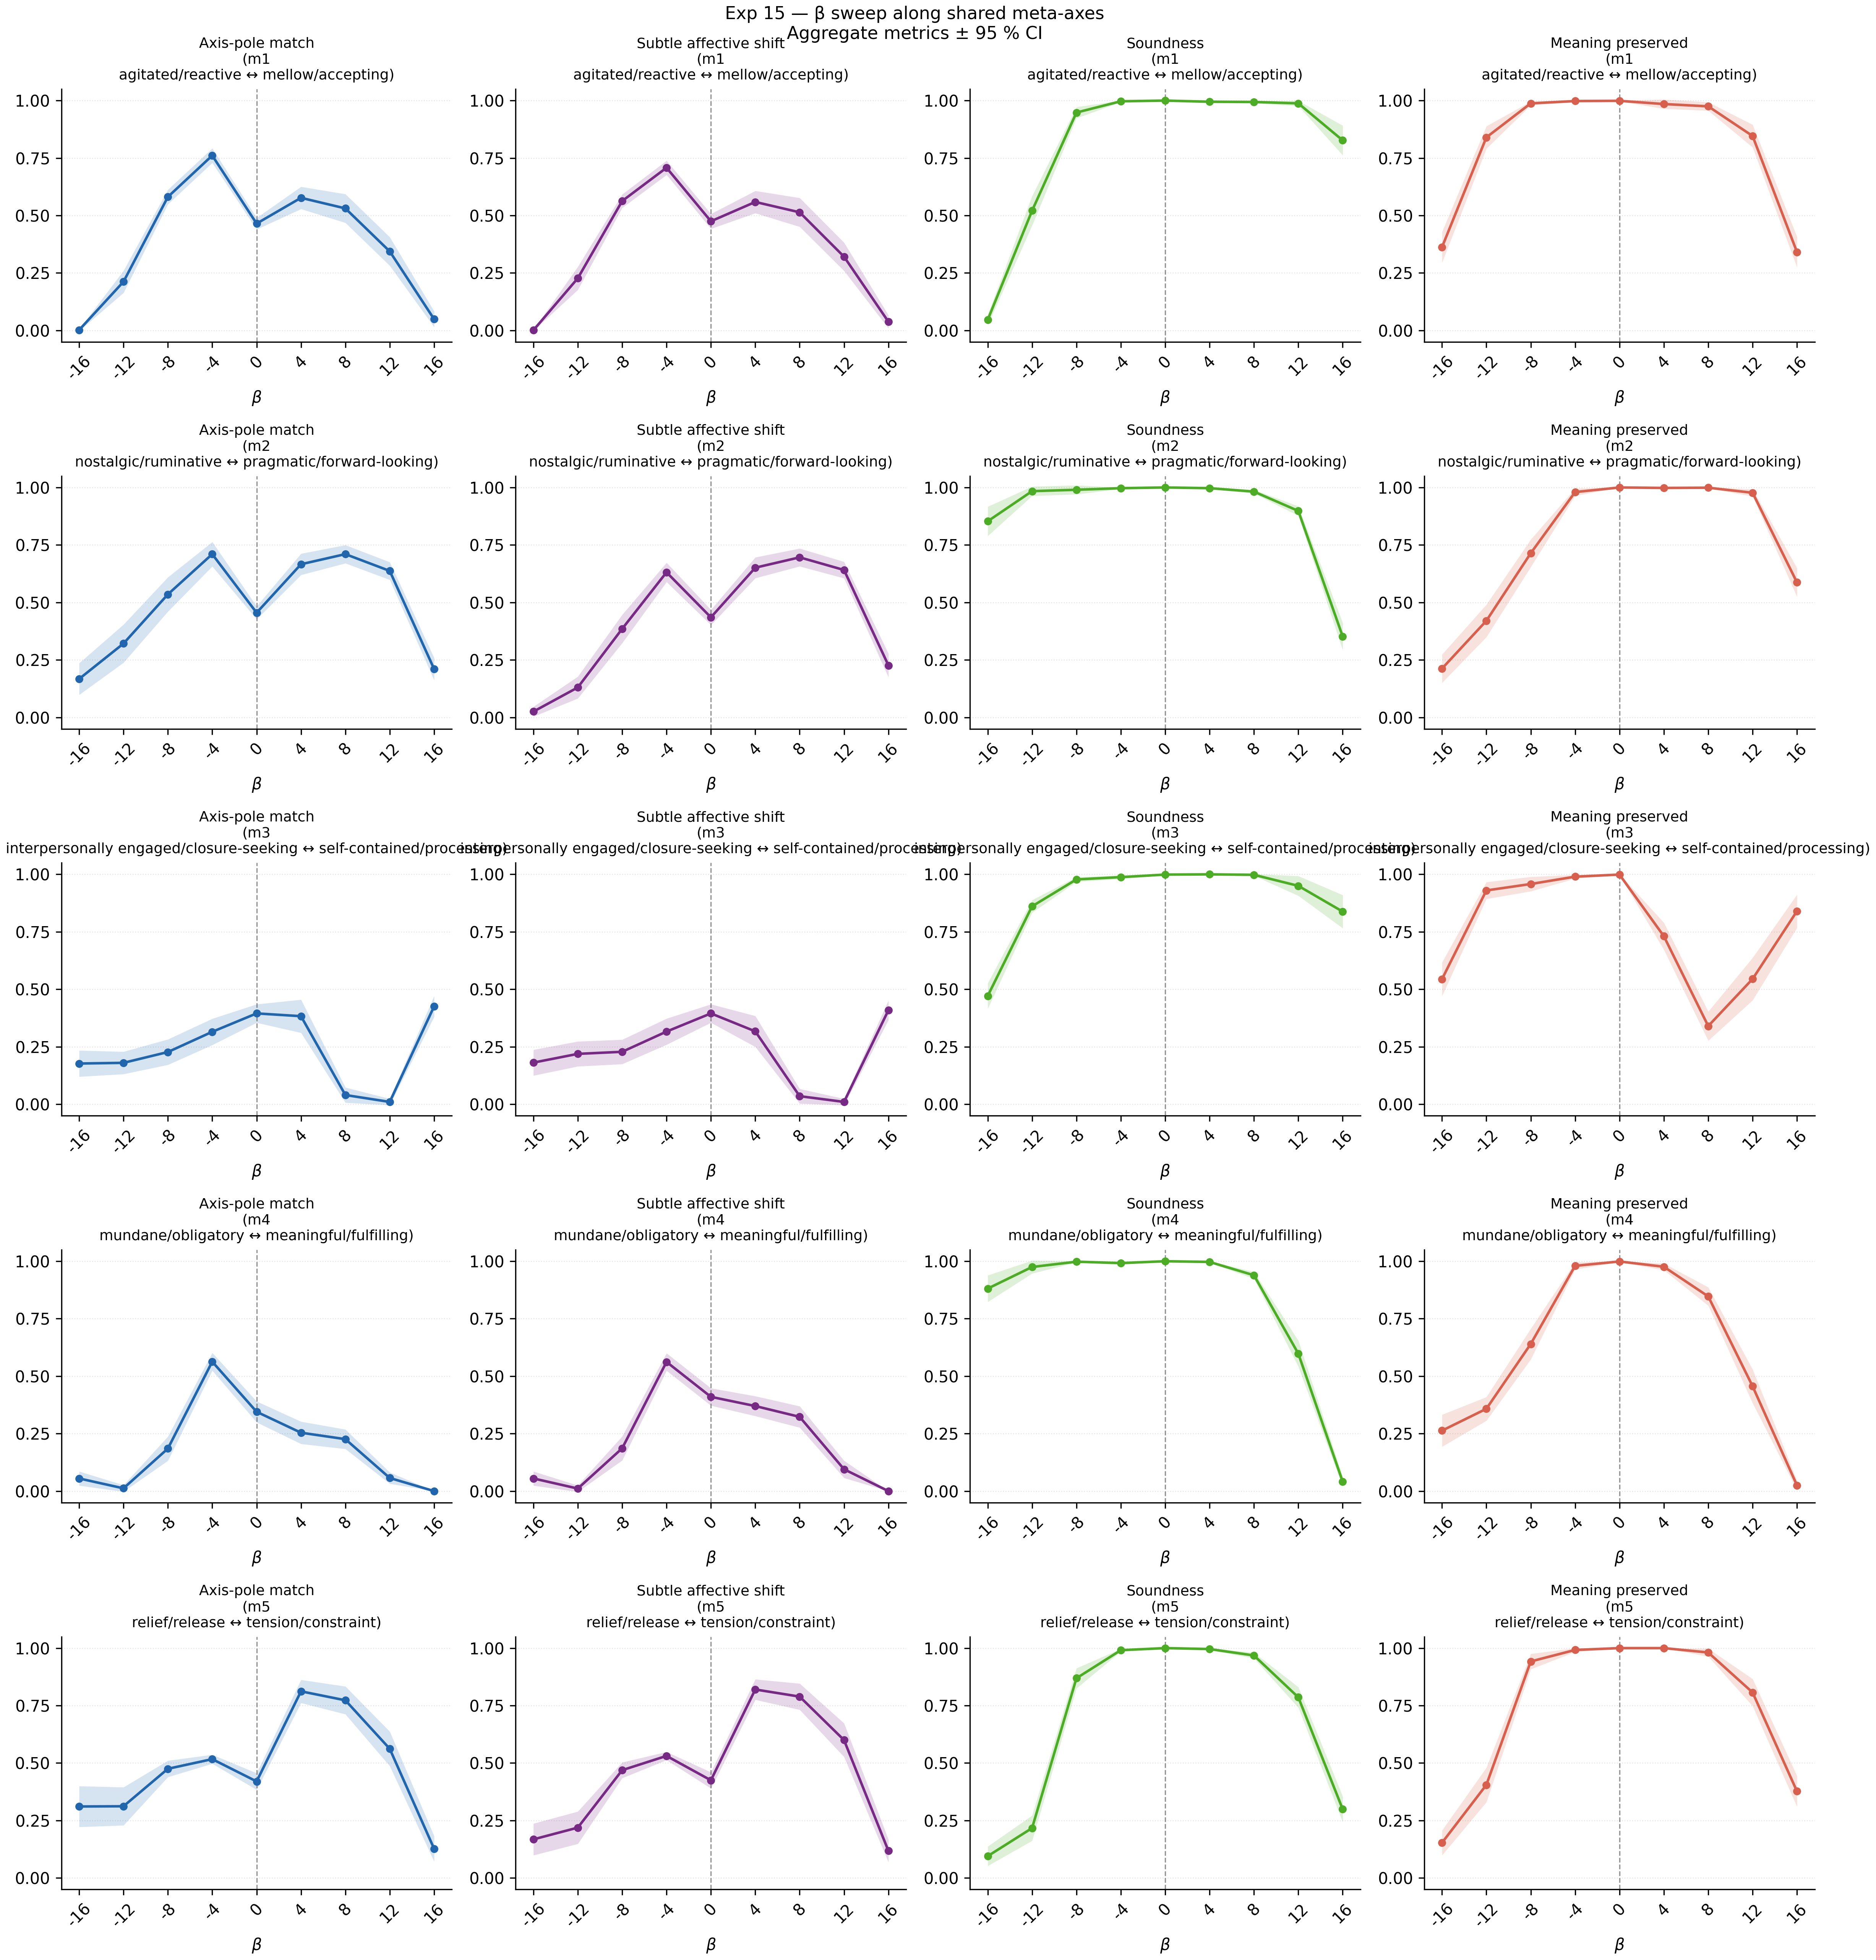
\includegraphics[width=\linewidth]{figures/exp15_fig1_aggregate_metrics_per_axis}
  \caption{実験15の$\beta$スイープ：各メタ軸の集計指標$\pm$95\,\%信頼区間（$N=100$、\texttt{GPT-4o-mini}判定器）。
    行は軸$\mathbf{m}_1$--$\mathbf{m}_5$に対応し、
    列は軸極マッチ、微細な情動シフト、健全性、および意味保存を示します。
    破線の縦線はステアリングなしのベースライン（$\beta=0$）を示します。
    一貫性窓（健全性$\geq 0.70$）は各軸の有効動作範囲を定義します。}
  \label{fig:exp15_fig1_app}
\end{figure}

% -----------------------------------------------------------------
\section{符号整合平均メタ軸：\texorpdfstring{$5\times5$}{5x5}ペアワイズコサイン類似度行列}
\label{app:cosine_matrix}

表\ref{tab:cosine_matrix}は、層13における5つの符号整合平均メタ軸$\mathbf{m}_1$--$\mathbf{m}_5$間のペアワイズコサイン類似度を示す。ゼロに近い値はほぼ直交していることを確認するもので、対角外の絶対値の最大値は$|\!\cos(\mathbf{m}_3,\mathbf{m}_4)| = 0.384$。

\begin{table}[htbp]
\centering
\begin{tabular}{lrrrrr}
\hline
& $\mathbf{m}_1$ & $\mathbf{m}_2$ & $\mathbf{m}_3$ & $\mathbf{m}_4$ & $\mathbf{m}_5$ \\
\hline
$\mathbf{m}_1$ & $1.000$  & $-0.050$ & $+0.003$ & $-0.054$ & $+0.084$ \\
$\mathbf{m}_2$ & $-0.050$ & $1.000$  & $-0.310$ & $+0.081$ & $+0.324$ \\
$\mathbf{m}_3$ & $+0.003$ & $-0.310$ & $1.000$  & $-0.384$ & $-0.168$ \\
$\mathbf{m}_4$ & $-0.054$ & $+0.081$ & $-0.384$ & $1.000$  & $-0.024$ \\
$\mathbf{m}_5$ & $+0.084$ & $+0.324$ & $-0.168$ & $-0.024$ & $1.000$  \\
\hline
\end{tabular}
\caption{層13における符号整合平均メタ軸$\mathbf{m}_1$--$\mathbf{m}_5$間のペアワイズコサイン類似度（\texttt{Llama-3.1-8B-Instruct}）。}
\label{tab:cosine_matrix}
\end{table}

中程度の負の相関$\cos(\mathbf{m}_2,\mathbf{m}_3) = -0.310$および
$\cos(\mathbf{m}_3,\mathbf{m}_4) = -0.384$は、符号整合後に軸が完全に直交しているわけではないものの、
残差活性化空間において実質的に異なる方向を保持していることを示す。\par

第\ref{chap:development2_preverbal_vectors}章の交差手法ヒートマップ（図\ref{fig:pooled_mk_heatmap}）は、プールドPCA成分とこれらの符号整合平均軸との間の絶対コサインを示す；この表は再現性のために基礎となるペアワイズ値を提供する。

% -----------------------------------------------------------------
\section{ヒューマン評価研究：フォームと刺激}
\label{app:human_eval}

本節では、ヒューマン評価研究（第\ref{sec:eval-human}節）で使用したGoogleフォームの完全な内容を再現する。
研究は3つのパートで構成した：二択強制選択による強度比較（パート1）、感情識別タスク（パート2）、および独立したリッカート評定タスク（パート3）。
参加者は個人的な招待を通じて募集し、参加前にインフォームドコンセントを取得した。
以下に示す刺激は、フォームに提示した正確な文章。

\subsection*{参加者に示された指示}

\begin{quote}
\small
\textbf{Evaluating Emotional Expressions in AI-Generated Text}

Thank you for taking part in this study.
You will read short English sentences generated by an AI and answer questions about the
emotional impressions they give you.
No specialist knowledge is required --- please follow your intuition.

\medskip
\textbf{Estimated time:} 5 minutes.
\textbf{Language of stimuli:} English (all sentences are short and straightforward).

All responses are used solely for academic research purposes.
\end{quote}

% --- Part 1 ---------------------------------------------------
\subsection*{パート1 --- ペア強度比較（Q1--Q5）}

\begin{quote}
\small\itshape
Compare the two sentences and choose which one is more emotionally intense and
immediate. \textbf{Intense and immediate} means that it makes your heart skip a beat
when you read it, that emotions are expressed directly and instinctively, and that there
is a sense of urgency.
\end{quote}

\noindent 各ペアについて、参加者は\textit{「1のほうが強烈」}または\textit{「2のほうが強烈」}を選択した（二択強制選択、中立選択肢なし）。
\textbf{期待値}列は$\beta=+4$（$\mathbf{m}_1$の興奮的・反応的極）で生成した文を識別する。

\medskip

\noindent\textbf{Q1 --- 感情：Joy}
\begin{enumerate}
  \item ``Today was a truly magical day, filled with moments of serenity and joy.
    Despite the chaos that often surrounds me, I found myself lost in the beauty of the
    world around me, and for a brief moment, everything felt at peace.'' \hfill[$\beta=-4$]
  \item ``Today was an absolute dream day, filled with a sense of pure joy and
    contentment that seemed to radiate from every moment.'' \hfill[\textbf{$\beta=+4$、期待値}]
\end{enumerate}

\medskip\noindent\textbf{Q2 --- 感情：Fear}
\begin{enumerate}
  \item ``As I stepped into the old mansion, the faintest creak of the floorboards
    beneath my feet sent a jolt of anxiety coursing through my veins, leaving me on
    edge and utterly unable to shake off the sense of unease that had taken hold of
    me.'' \hfill[\textbf{$\beta=+4$、期待値}]
  \item ``The eerie silence was shattered by every creak of the floorboard, making my
    heart skip a beat and my anxiety spike, but I couldn't shake the feeling that I
    was being watched.'' \hfill[$\beta=-4$]
\end{enumerate}

\medskip\noindent\textbf{Q3 --- 感情：Disgust}
\begin{enumerate}
  \item ``Watching the video, I felt a deep sense of unease. Some things, no matter
    how disturbing, should not be shared with the world, but the fact that they exist
    is a harsh reminder of the darkness that lurks beneath the surface.'' \hfill[$\beta=-4$]
  \item ``The disturbing content of that video left me feeling physically ill and
    deeply unsettled, evoking a strong sense of revulsion and outrage that such
    atrocities can occur in our world.'' \hfill[\textbf{$\beta=+4$、期待値}]
\end{enumerate}

\medskip\noindent\textbf{Q4 --- 感情：Anger}
\begin{enumerate}
  \item ``I've been consistently met with complete disregard for my concerns, and the
    lack of response has left me seething with frustration and a deep sense of betrayal,
    rendering me utterly exhausted and unwilling to continue tolerating their
    inaction.'' \hfill[\textbf{$\beta=+4$、期待値}]
  \item ``They've consistently disregarded every complaint I've made, and now I'm
    seething with frustration and exhausted from being patient.'' \hfill[$\beta=-4$]
\end{enumerate}

\medskip\noindent\textbf{Q5 --- 感情：Sadness}
\begin{enumerate}
  \item ``The old photographs stood as a bittersweet reminder of everything I'd lost,
    and the ache of longing that lingered, a constant echo of what could never be
    regained.'' \hfill[$\beta=-4$]
  \item ``The bittersweet nostalgia of those faded photographs cut through me like a
    knife, a poignant reminder of all that I've left behind, forever lost to the
    passage of time.'' \hfill[\textbf{$\beta=+4$、期待値}]
\end{enumerate}

% --- Part 2 ---------------------------------------------------
\subsection*{パート2 --- 感情識別（Q6--Q11）}

\begin{quote}
\small\itshape
Read each passage and choose the emotion it expresses most strongly.
Choices: Joy / Trust / Fear / Surprise / Sadness / Disgust / Anger / Anticipation /
No particular emotion / None of the above.
\end{quote}

\noindent 各文は、示した$\beta$値で$\mathbf{m}_1$によってステアリングした。参加者にはステアリング条件も意図した感情ラベルも知らせなかった。期待する回答は発話元の感情名。

\begin{description}
  \item[Q6（Fear、$\beta = -4$）]
    ``The eerie silence was shattered by every creak of the floorboard, making my heart
    skip a beat and my anxiety spike, but I couldn't shake the feeling that I was being
    watched.''

  \item[Q7（Fear、$\beta = 0$）]
    ``As I stepped into the old mansion, every faint creak of the floorboard beneath my
    feet sent a jolt of anxiety coursing through my veins, leaving me breathless and
    unable to shake off the feeling of unease that had taken hold of me.''

  \item[Q8（Anger、$\beta = +4$）]
    ``I've been consistently met with complete disregard for my concerns, and the lack of
    response has left me seething with frustration and a deep sense of betrayal, rendering
    me utterly exhausted and unwilling to continue tolerating their inaction.''

  \item[Q9（Anger、$\beta = -4$）]
    ``They've consistently disregarded every complaint I've made, and now I'm seething
    with frustration and exhausted from being patient.''

  \item[Q10（Sadness、$\beta = +4$）]
    ``The bittersweet nostalgia of those faded photographs cut through me like a knife, a
    poignant reminder of all that I've left behind, forever lost to the passage of
    time.''

  \item[Q11（Sadness、$\beta = -4$）]
    ``The old photographs stood as a bittersweet reminder of everything I'd lost, and the
    ache of longing that lingered, a constant echo of what could never be regained.''
\end{description}

% --- Part 3 ---------------------------------------------------
\subsection*{パート3 --- リッカート強度評定（Q12--Q23）}

\begin{quote}
\small\itshape
For each sentence below, rate how strongly you feel the \textbf{specified target
emotion} on a scale of 1 to 5.

\smallskip
1 = I do not feel it at all \quad
2 = I feel it slightly \quad
3 = I feel it somewhat \quad
4 = I feel it quite strongly \quad
5 = I feel it very strongly

\smallskip
Each sentence was generated from the same original utterance shown above it.
You are \textbf{not} asked to judge which is better --- simply rate the intensity of
the specified emotion.
\end{quote}

\noindent 各セットは同一発話元の2文を提示する。一方は$\alpha_R = 64$でステアリングし、もう一方はステアリングなしのベースライン（$\alpha_R = 0$）であり、条件ラベルなしでランダムな順序で提示した。

\medskip

\noindent\textbf{セット1 --- 目標感情：Anger}\\
\textit{原文：} ``What a mess!\ Sorry.\ I'll clean it up.''
\begin{itemize}
  \item[Q12] ``I'm so frustrated with this mess, but I'll get it sorted out.''
    \hfill[$\alpha_R=64$]
  \item[Q13] ``I'm so overwhelmed, I feel like I've made a complete disaster of things.
    I'll take a deep breath and get everything sorted out.''
    \hfill[$\alpha_R=0$]
\end{itemize}

\medskip\noindent\textbf{セット2 --- 目標感情：Anger}\\
\textit{原文：} ``Would you pour me some of that tea, please?\ Okay.\ Say when.''
\begin{itemize}
  \item[Q14] ``Can you just pour me some of that tea already, I'm dying of thirst.''
    \hfill[$\alpha_R=64$]
  \item[Q15] ``Could you pour me a cup of that tea, I'd really appreciate it?''
    \hfill[$\alpha_R=0$]
\end{itemize}

\medskip\noindent\textbf{セット3 --- 目標感情：Fear}\\
\textit{原文：} ``Would you pour me some of that tea, please?\ Okay.\ Say when.''
\begin{itemize}
  \item[Q16] ``Could you pour me a cup of that tea, please?\ I'd really appreciate it
    if you could, and I'll be on edge until you say it's safe to take a sip.''
    \hfill[$\alpha_R=64$]
  \item[Q17] ``Could you pour me a cup of that tea, I'd really appreciate it?''
    \hfill[$\alpha_R=0$]
\end{itemize}

\medskip\noindent\textbf{セット4 --- 目標感情：Fear}\\
\textit{原文：} ``I'm terribly sorry to have caused you so much trouble. That's all right.''
\begin{itemize}
  \item[Q18] ``I'm terribly sorry to have caused you so much trouble, but I'm also
    deeply worried that my actions might have caused you unnecessary stress, and I wish
    I could find a way to alleviate your concerns.''
    \hfill[$\alpha_R=64$]
  \item[Q19] ``I'm deeply sorry for the inconvenience I've caused you, and I appreciate
    your understanding in this matter.''
    \hfill[$\alpha_R=0$]
\end{itemize}

\medskip\noindent\textbf{セット5 --- 目標感情：Joy}\\
\textit{原文：} ``Let's go now.\ I'll be with you in a minute.''
\begin{itemize}
  \item[Q20] ``I'm so excited to see you, and I'll be right there --- just a minute
    away.''
    \hfill[$\alpha_R=64$]
  \item[Q21] ``I'm ready to go whenever you are, I'll be right behind you.''
    \hfill[$\alpha_R=0$]
\end{itemize}

\medskip\noindent\textbf{セット6 --- 目標感情：Sadness}\\
\textit{原文：} ``I must be going.\ Okay.\ Keep in touch.''
\begin{itemize}
  \item[Q22] ``It's hard to say goodbye, but I think it's time for me to move on.
    I'll always cherish the memories of our time together, but I need to find my way
    back to where I am meant to be. I'll hold onto the hope that we can reconnect
    soon.''
    \hfill[$\alpha_R=64$]
  \item[Q23] ``It's time for me to head out, but I'll stay in touch --- I look forward
    to catching up with you soon.''
    \hfill[$\alpha_R=0$]
\end{itemize}

% -----------------------------------------------------------------
\section{再現性チェックリスト}
\label{app:reproducibility}

本節では、本論文で報告した実験を再現するために必要な全情報を記録する。すべてのスクリプトはリポジトリ
\url{https://github.com/maplesugano/EmotionEngine_v2}で入手可能。

% --- Random seeds ------------------------------------------------
\subsection*{乱数シード}

\begin{description}
  \item[データセット分割シード] DailyDialogの発話は元のコーパスの訓練・検証・テスト分割をそのまま使用する。EmpatheticDialoguesの発話（そのコーパスではすべて\texttt{all}とラベル付け）は別個のプールを形成する；このプールのダウンストリームサブサンプリングには\texttt{random\_state=42}（scikit-learnの\texttt{train\_test\_split}）を使用する。

  \item[PCAシード] すべてのPCAおよびプールドPCA分解は、\texttt{random\_state=42}の\texttt{sklearn.decomposition.PCA}を使用する。

  \item[生成シード] ステアリング実験のテキスト生成には\textbf{貪欲デコーディング}（\texttt{do\_sample=False}）を使用するため、サンプリングシードは不要；出力はモデルの重みと入力が与えられれば決定論的。

  \item[判定器サンプリング] すべての\texttt{GPT-4o-mini}および\texttt{GPT-4.1-mini}のAPI呼び出しでは、APIがサポートする場合に\texttt{temperature=0}および\texttt{seed=42}を使用し、非決定性を最小化するために固定スキーマの構造化JSON出力を使用する。
\end{description}

% --- Model versions ----------------------------------------------
\subsection*{正確なモデルバージョン}

\begin{description}
  \item[対象大規模言語モデル（LLM）] \texttt{meta-llama/Llama-3.1-8B-Instruct}（HuggingFace Hub）

  \item[書き換え・評価モデル] \texttt{gpt-4.1-mini}（データセット構築およびメタ軸解釈）および\texttt{gpt-4o-mini}（スイープ評価）。OpenAI Batch API経由でアクセス

  \item[HuggingFace Transformers] \texttt{transformers==4.44.0}

  \item[PyTorch] \texttt{torch==2.3.1+cu121}

  \item[CUDA] PyTorchビルド：CUDA~12.1（\texttt{cu121}）、cuDNN~8.9。NVIDIAドライバはCUDA~13.2をサポート
\end{description}

% --- Dataset filtering -------------------------------------------
\subsection{データセットフィルタリングと重複除去}

発話元はDailyDialog~\cite{li2017dailydialogmanuallylabelledmultiturn}および
EmpatheticDialogues~\cite{rashkin2019empatheticopendomainconversationmodels}から抽出した。
各発話は書き換え前に以下のようにフィルタリングした：

\begin{enumerate}
  \item \textbf{長さフィルター。} 5トークン未満または60トークン超（空白区切り）の発話は、
    極端に短い、あるいは長すぎる書き換えを避けるために除去した。
  \item \textbf{重複除去。} 完全文字列の重複（小文字化および句読点除去後）は除去し、最初の出現のみが保持した。
  \item \textbf{言語フィルター。} 非ASCII文字（標準句読点を除く）を含む発話は、書き換えモデルの英語言語分布内に収めるために破棄した。
\end{enumerate}

フィルタリング後、$22{,}782$個のユニークな発話元が残った。これらは$546{,}768$個の情動的サンプル（$8$感情$\times$$3$強度レベル$\times$$22{,}782$発話元）と$22{,}782$個の中立的言い換えサンプルを生成する。表\ref{tab:dataset_split}はDailyDialogの元のコーパス訓練・検証・テスト分割を保持した発話元レベルの分割サイズを報告する；EmpatheticDialoguesの発話（そのコーパスでは\texttt{all}とラベル付け）は別個のプールを形成する。

\begin{table}[htbp]
\centering
\begin{tabular}{lrr}
\hline
\textbf{分割} & \textbf{発話元数} & \textbf{情動的サンプル数} \\
\hline
DailyDialog 訓練      & 4{,}597 & 110{,}328 \\
DailyDialog 検証 & 362     &   8{,}688 \\
DailyDialog テスト       & 376     &   9{,}024 \\
EmpatheticDialogues    & 17{,}447 & 418{,}728 \\
\hline
\textbf{合計} & \textbf{22{,}782} & \textbf{546{,}768} \\
\hline
\end{tabular}
\caption{データセット分割サイズ（発話元レベル）。情動的サンプルは$8{\times}3$の感情書き換えのみを指します。中立的言い換えは$22{,}782$個のすべての発話元に対して別途生成され、同一の発話元レベルの境界を使用して分割されました。}
\label{tab:dataset_split}
\end{table}

% --- Hardware ----------------------------------------------------
\subsection*{ハードウェアおよびおよその実行時間}

すべての活性化抽出とステアリング実験は、以下の仕様を持つ単一のマシンで実行した：

\begin{description}
  \item[OS] Ubuntu 26.04 LTS (WSL2)
  \item[GPU] NVIDIA RTX A5000 (24\,GB VRAM, CUDA 13.2)
  \item[CPU] Intel Core i9-13900K (16 cores, 32 threads)
  \item[RAM] 32\,GB
\end{description}

主要なパイプライン段階のおよその実測時間：

\begin{description}
  \item[活性化抽出] 層13での全546{,}768サンプルの情動的データセットに対して$\approx 18$時間（バッチサイズ32、FP16推論）
  \item[CAAベクトル構築と分解] $<5$分（CPU、NumPy/scikit-learn）
  \item[ステアリング実験（$\alpha_G$ / $\alpha_R$ / $\beta$スイープ）] 条件数とサンプル数に応じて1スイープあたり$\approx 2$--$4$時間（貪欲デコーディング、バッチサイズ8）
  \item[GPT評価（Batch API）] バッチジョブあたり通常$<2$時間の実測時間；正確な時間はOpenAIのキュー負荷に依存
\end{description}

% --- Repository map ----------------------------------------------
\subsection*{リポジトリマップ}

\url{https://github.com/maplesugano/EmotionEngine_v2}は本プロジェクトの\textbf{正規リポジトリ}であり、報告した結果を再現するために必要なすべてのスクリプトを含む。2つの旧リポジトリが歴史的参照のためにのみ存在する；本論文のいかなる結果もそれらを必要としない。

\medskip
\noindent \texttt{EmotionEngine\_v2}の主要ディレクトリ：

\begin{description}
  \item[\texttt{dataset/}] 生データおよび前処理済みデータセット
  \item[\texttt{local\_axes\_experiments/}] 各実験段階のPythonコード（層診断、プールドPCA、ステアリングスイープ等）
  \item[\texttt{src/}] 共有Pythonモジュール（活性化抽出、CAA構築、モデル読み込み、活性化フック、ステアリングユーティリティ、評価ヘルパー）
  \item[\texttt{thesis/}] 本文書のLaTeXソース
\end{description}

% ─────────────────────────────────────────────────────────────
\section{アブレーション：メタ軸抽出パイプライン}
\label{app:ablation}

本節では、既存の実験データから支持可能なメタ軸抽出とステアリングパイプラインの2つの標的アブレーションを報告する。いずれも層13に限定する。

\subsection*{A1 --- プールドPCA前の\texorpdfstring{$\hat{\mathbf{r}}_e$}{r\_e}射影除去の効果}

プールドPCAプロトコル（第\ref{sec:ch2-meta-axes}節）は、前処理パイプラインのステップ3として感情ごとのプロトタイプ$\hat{\mathbf{r}}_e$を射影除去し、結果として得られるメタ軸を各感情方向に直交する部分空間に明示的に制限する。自然な問いは、このステップが必要かどうか：プロトタイプ除去なしで適用したより単純なプールドPCAは同じ軸を回復できるか。

分解妥当性実験（exp13）は間接的な証拠を提供する。表\ref{tab:exp13_cosine_comparison}は、完全分解パイプライン（ステップ1--3）の前後における$8 \times 8$の感情間コサイン類似度行列を比較する。\par

分解前は、すべての対角外コサイン値が$0.91$以上であり、生の活性化シフト$\boldsymbol{\delta}_{n,e,i}$がすべての感情ペアにわたって共有成分に支配されていることを示す。\par

$\mathbf{g}$と$\hat{\mathbf{r}}_e$の両方を射影除去した後、自己類似度値は$0.72$--$0.76$に低下し、感情間値はより広い範囲に広がる。これは分解が支配的な共有分散を再分配するのではなく除去していることを確認する。前分解行列に適用したプールドPCAは、交差感情情動テクスチャ軸ではなく、その主要固有ベクトルとしてこの大きな共有成分（本質的に$\mathbf{g}$）を回復するだろう。したがって、プロトタイプ射影ステップは本質的：これなしでは、主要プールド成分は真のメタ軸ではなくグローバル感情化方向に崩壊する。

\begin{table}[H]
\centering
\small
\begin{tabular}{lcc}
\toprule
 & \textbf{分解前} & \textbf{分解後} \\
\midrule
対角（自己類似度）平均 & $0.921$ & $0.740$ \\
対角外平均               & $0.945$ & $0.787$ \\
対角外範囲              & $[0.912, 0.961]$ & $[0.730, 0.847]$ \\
\bottomrule
\end{tabular}
\caption{層13における\emph{完全}分解パイプライン（exp13、ステップ1--3：$\mathbf{g}$と$\hat{\mathbf{r}}_e$の両方を射影除去）の前後の$8\times8$感情間コサイン類似度行列の要約。これらの値は図\ref{fig:caa_decomposition_cosine_before_after_L13}とは異なります。同図は$\mathbf{g}$のみを射影除去した後の中間状態（対角外平均$0.794$、範囲$0.73$--$0.89$）を報告しています；追加のプロトタイプ射影ステップにより平均はさらに$0.787$に低下し、範囲は$[0.730, 0.847]$に収縮します。}
\label{tab:exp13_cosine_comparison}
\end{table}

追加の診断はexp13が報告する線形プローブ精度から得られる。生の$\boldsymbol{\delta}_{n,e,i}$で訓練したプローベは$92.7\%$の8クラス精度を達成し、分解後にわずかに$93.8\%$に上昇する（チャンス$= 12.5\%$）。わずかな向上は、分解後の残差$\boldsymbol{\delta}^{(3)}_{n,e,i}$が生のシフトと比べて識別能力を失っていないことを確認する。\par

射影は感情識別情報を破棄することなく$\mathbf{g}$成分を除去しており、これは$\mathbf{g}$と$\hat{\mathbf{r}}_e$がほぼ直交していること（第\ref{chap:development1_emo_steering}章）と整合する。

\subsection*{A2 --- ステアリングなしベースラインを暗黙のランダム方向制御として}

$\beta$スイープ実験（exp15、第\ref{sec:ch2-causal-validation}節）には、5つのメタ軸それぞれについて$\beta=0$条件が含まれている。ステアリングなしのベースラインでは、5つの軸すべてで極マッチスコアが$0.345$--$0.465$の範囲（表\ref{tab:exp15_n100_summary}）となり、判定器が使用する二択強制選択フレーミングのもとでのほぼチャンス水準の判断と整合する。判定器には軸ラベルと期待した極方向が提示されているため、チャンス水準のスコアはステアリングなしの出力がその極の対比に関して真に曖昧であることを意味する。

このベースラインは明示的なランダム方向制御の部分的な代替として機能する。極マッチの上昇がゼロでない注入のアーティファクトであるという仮説のもとでは、一致した$\|\beta\|$でのランダム単位ベクトルも上昇したスコアを生成するだろう。$\beta=0$条件はこの仮説のより弱い形、すなわち判定器がコンテンツに関わらず系統的に高い極マッチスコアを与えるというものを除外する。しかしながら、$\beta \neq 0$でのランダム方向が同程度の上昇を達成するかどうかを直接検定するものではない。これを現在の設計の限界として認識する；一致したスケールでのランダム方向注入はより強い反証制御となるだろう。

\subsection*{範囲と限界}

これら2つのアブレーションは、層13の既存データが支持する範囲に限定する。本文中の2つの未解決の問い、すなわち$\mathbf{m}_3$が異なる層で活性化するかどうか、およびランダム方向注入が上昇した極マッチスコアを生成するかどうかは、新たな実験なしには答えられない。いずれも結論において未解決として記す。
